\documentclass{beamer}
\usepackage{../../shared/styles/custom}


%\beamerdefaultoverlayspecification{<+->}
% \newcommand{\data}{\mathcal{D}}
% \newcommand\Item[1][]{%
% 	\ifx\relax#1\relax  \item \else \item[#1] \fi
% 	\abovedisplayskip=0pt\abovedisplayshortskip=0pt~\vspace*{-\baselineskip}}




\title{Logistic Regression}
\date{\today}
\author{Nipun Batra}
\institute{IIT Gandhinagar}
\begin{document}
	\maketitle

	\section{Problem Setup}
	
	\begin{frame}{Classification Technique}
	%\vspace{5cm}
	\begin{minipage}{0.3\textwidth}
		% Show the image at item three and afterwards
		
		\begin{figure}
			
			% From https://i.imgur.com/AyzVOIO.jpg
			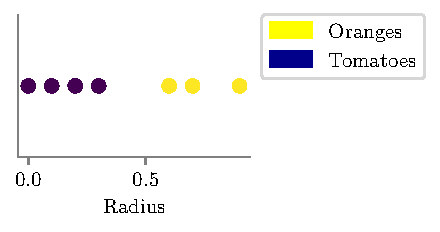
\includegraphics{../figures/logistic-regression/logistic-orange-tomatoes-original.pdf}
		\end{figure}
	\end{minipage} \\

	
\end{frame}
	
	\begin{frame}{Classification Technique}
	%\vspace{5cm}
	\begin{minipage}{0.3\textwidth}
		% Show the image at item three and afterwards
		
		\begin{figure}
			
			% From https://i.imgur.com/AyzVOIO.jpg
			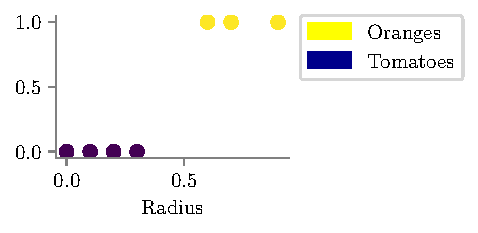
\includegraphics{../figures/logistic-regression/logistic-orange-tomatoes.pdf}
		\end{figure}
	\end{minipage} \\
	%\vspace{-1.7cm}
	\pause Aim: Probability(Tomatoes $|$ Radius) ? or
	\pause \framebox{More generally, P($y = 1 | X = x$)?}
	
\end{frame}

\begin{frame}{Idea: Use Linear Regression}
\hspace{2.5cm}
\begin{minipage}{0.3\textwidth}
	% Show the image at item three and afterwards
	
	\begin{figure}
		
		% From https://i.imgur.com/AyzVOIO.jpg
		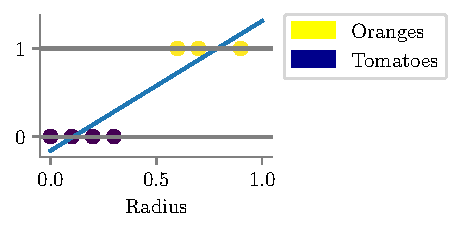
\includegraphics{../figures/logistic-regression/linear-orange-tomatoes.pdf}
	\end{figure}
\end{minipage} \\
\begin{equation*}
P(X = Orange | Radius) = \theta_{0} + \theta_{1} \times Radius
\end{equation*}
\pause Generally,
\begin{equation*}
P(y = 1 | x) = X\theta
\end{equation*}
\end{frame}
\begin{frame}{Idea: Use Linear Regression}
Prediction:\\
If $\theta_{0} + \theta_{1}\times Radius > 0.5 \rightarrow$ Orange \\
\hspace{3.3cm} Else $\rightarrow$ Tomato\\
Problem:\\
Range of $X\theta$ is $(-\infty, \infty)$\\
But $P(y = 1 | \ldots) \in [0, 1]$
\end{frame}

\begin{frame}{Idea: Use Linear Regression}
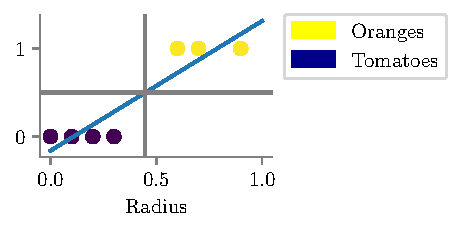
\includegraphics{../figures/logistic-regression/linear-orange-tomatoes-decision.pdf}
\end{frame}

\begin{frame}{Idea: Use Linear Regression}
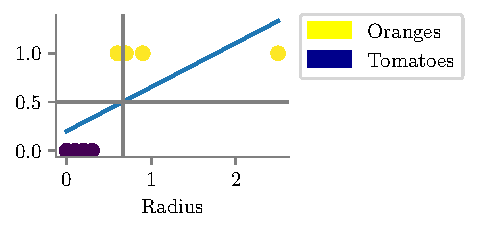
\includegraphics{../figures/logistic-regression/linear-orange-tomatoes-decision-modified.pdf}


Linear regression for classification gives a poor prediction!
\end{frame}

\begin{frame}{Ideal boundary}
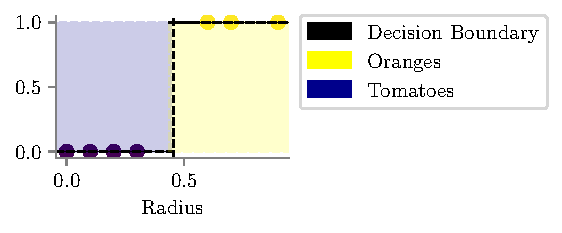
\includegraphics{../figures/logistic-regression/linear-orange-tomatoes-decision-ideal.pdf}

\begin{itemize}[<+->]
	\item Have a decision function similar to the above (but not so sharp and discontinuous)
	\item Aim: use linear regression still!
\end{itemize}
\end{frame}

\begin{frame}{Idea: Use Linear Regression}
\hspace{1cm}
\begin{minipage}{0.3\textwidth}
% Show the image at item three and afterwards
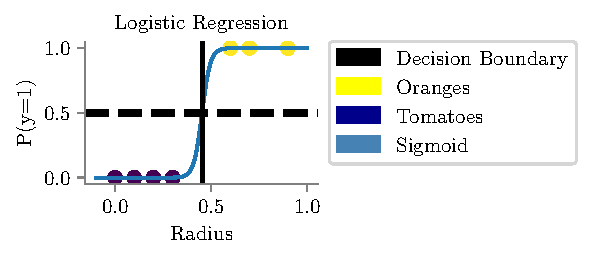
\includegraphics{../figures/logistic-regression/logistic.pdf}
\end{minipage} \\
Question. Can we still use Linear Regression? \\
Answer. Yes! Transform $\hat{y} \rightarrow [0, 1]$
\end{frame}

\section{Logistic/Sigmoid function}

\begin{frame}{Logistic / Sigmoid Function}
$\hat{y} \in (-\infty, \infty)$ \\
$\phi =$ Sigmoid / Logistic Function $(\sigma)$ \\
$\phi(\hat{y}) \in [0, 1]$
\begin{equation*}
\sigma(z) = \frac{1}{1 + e^{-z}}
\end{equation*}
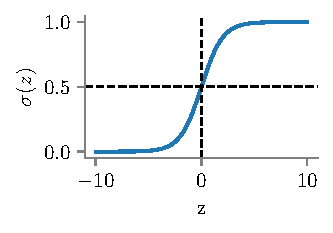
\includegraphics{../figures/logistic-regression/logistic-function.pdf}
\end{frame}

\begin{frame}{Logistic / Sigmoid Function}
 $z \rightarrow \infty$\\
\pause  $\sigma(z) \rightarrow 1$\\
\pause $z \rightarrow -\infty$\\
 \pause $\sigma(z) \rightarrow 0$\\
 \pause $z = 0$\\
 \pause $\sigma(z) = 0.5$

\end{frame}

\begin{frame}{Logistic / Sigmoid Function}
Question. Could you use some other transformation $(\phi)$ of $\hat{y}$ s.t. \\
\begin{equation*}
\phi(\hat{y}) \in [0, 1]
\end{equation*}
Yes! But Logistic Regression works.
\end{frame}
\begin{frame}{Logistic / Sigmoid Function}
\begin{equation*}
P(y = 1 | X) = \sigma(X\theta) = \frac{1}{1 + e^{-X\theta}}    
\end{equation*}
Q. Write $X\theta$ in a more convenient form (as $P(y = 1|X)$, $P(y = 0 | X)$)\\
\end{frame}
\begin{frame}{Logistic / Sigmoid Function}
\begin{equation*}
P(y = 1 | X) = \sigma(X\theta) = \frac{1}{1 + e^{-X\theta}}    
\end{equation*}
Q. Write $X\theta$ in a more convenient form (as $P(y = 1|X)$, $P(y = 0 | X)$)\\
\pause \begin{equation*}
P(y = 0 | X) = 1 - P(y = 1 | X) = 1 - \frac{1}{1 + e^{-X\theta}} = \frac{e^{-X\theta}}{1 + e^{-X\theta}} 
\end{equation*}

\pause \begin{equation*}
\therefore \frac{P(y = 1|X)}{1 - P(y = 1|X)} = e^{X\theta}
\implies X\theta = \log\frac{P(y = 1|X)}{1 - P(y = 1 | X)}
\end{equation*}
\end{frame}
\begin{frame}{Odds (Used in betting)}
$$\frac{P(win)}{P(loss)}$$ \\
\hspace{3cm} Here,\\
$$Odds = \frac{P(y = 1)}{P(y = 0)}$$ \\
\centering
\framebox{log-odds = $\log\frac{P(y = 1)}{P(y = 0)} = X\theta$}
\end{frame}
\begin{frame}{Logistic Regression}
Q. What is decision boundary for Logistic Regression?
\end{frame}
\begin{frame}{Logistic Regression}
Q. What is decision boundary for Logistic Regression? \\
\hspace{0.4cm} Decision Boundary: $P(y = 1|X) = P(y = 0 | X)$\\
\vspace{0.3cm}
\hspace{4cm} or $\frac{1}{1 + e^{-X\theta}} = \frac{e^{-X\theta}}{1 + e^{-X\theta}}$  \\
\vspace{0.3cm}
\hspace{4cm} or $e^{X\theta} = 1$\\
\vspace{0.3cm}
\hspace{4cm} or $X\theta = 0$
\end{frame}
\begin{frame}{Learning Parameters}
Could we use cost function as:
\begin{equation*}
J(\theta) = \sum (y_{i} - \hat{y}_{i})^{2}
\end{equation*}
\begin{equation*}
\hat{y}_{i} = \sigma(X\theta)
\end{equation*}
Answer: No (Non-Convex) \\ \hspace{1.2cm} (See Jupyter Notebook)
\end{frame}


\section{Deriving Cost Function via Maximum Likelihood Estimation}

\begin{frame}{Cost function convexity}
\begin{columns}
	\begin{column}{0.5\textwidth}
		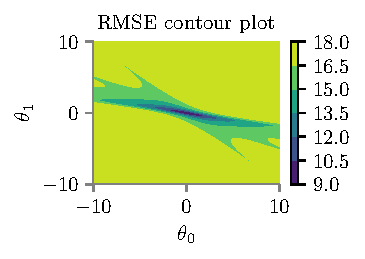
\includegraphics[scale=0.7]{../figures/logistic-regression/logistic-sse-loss-contour.pdf}
	\end{column}
\begin{column}{0.5\textwidth}
	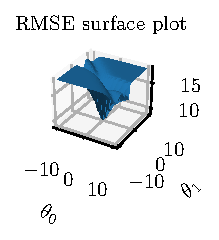
\includegraphics[scale=0.7]{../figures/logistic-regression/logistic-sse-loss-3d.pdf}
\end{column}
\end{columns}
\end{frame}

\begin{frame}{Learning Parameters}
Likelihood = $P(D | \theta)$ \\
\vspace{0.2cm}
$P(y | X, \theta) = \prod_{i=1}^{n} P(y_{i} | x_{i}, \theta)$ \\ where y = 0 or 1
\end{frame}
\begin{frame}{Learning Parameters}
Likelihood = $P(D | \theta)$ \\
\vspace{-0.4cm}
\begin{align*}
P(y | X, \theta) &= \prod_{i=1}^{n} P(y_{i} | x_{i}, \theta) \\ &= \prod_{i=1}^{n} \Big\{\frac{1}{1 + e^{-x_{i}^{T}\theta}}\Big\}^{y_{i}}\Big\{1 - \frac{1}{1 + e^{-x_{i}^{T}\theta}}\Big\}^{1 - y_{i}} \\
\end{align*}
\vspace{0.2cm}
[Above: Similar to $P(D|\theta)$ for Linear Regression; \\
\hspace{1.3cm} Difference Bernoulli instead of Gaussian]\\
\begin{align*}
-\log P(y | X, \theta) &= \text{Negative Log Likelihood}\\ &= \text{Cost function will be minimising} \\ &= J(\theta)
\end{align*}
\end{frame}


%\begin{frame}{Likelihood Visualisation}
%\includegraphics{../figures/logistic-regression/logistic-likelihood.pdf}
%\end{frame}

\begin{frame}{Aside on Bernoulli Likelihood}
\begin{itemize}[<+->]
\item Assume you have a coin and flip it ten times and get (H, H, T, T, T, H, H, T, T, T).
\item What is p(H)?
\item We might think it to be: 4/10 = 0.4. But why?
\item Answer 1: Probability defined as a measure of long running frequencies
\item Answer 2: What is likelihood of seeing the above sequence when the p(Head)=$\theta$?
\item Idea find MLE estimate for $\theta$
\end{itemize}

\end{frame}

\begin{frame}{Aside on Bernoulli Likelihood}
\begin{itemize}[<+->]
\item $p(H) = \theta$ and $p(T) = 1 - \theta$
\item What is the PMF for first observation $P(D_1 = x|\theta)$, where x = 0 for Tails and x = 1 for Heads?
\item $P(D_1 = x|\theta) = \theta^x(1-\theta)^{(1-x)}$
\item Verify the above: if x = 0 (Tails), $P(D_1 = x|\theta) = 1 - \theta$ and if x = 1 (Heads), $P(D_1 = x|\theta)  = \theta$
\item What is $P(D_1, D_2, ..., D_n|\theta)$?
\item $P(D_1, D_2, ..., D_n|\theta) = P(D_1\theta)P(D_2|\theta)...P(D_n|\theta)$
\item $P(D_1, D_2, ..., D_n|\theta) =\theta^{n_h}(1-\theta)^{n_t}$
\item Log-likelihood = $\mathcal{LL}(\theta) = n_h\log(\theta) + n_t\log(1-\theta)$
\item $\frac{\partial \mathcal{LL}(\theta)}{\partial \theta} = 0 \implies \frac{n_h}{\theta} + \frac{n_t}{1-\theta} = 0 \implies \theta_{MLE} = \frac{n_h}{n_h + n_t}$

\end{itemize}

\end{frame}

\section{Cross Entropy Cost Function}
\begin{frame}{Learning Parameters}
\begin{align*}
J(\theta) &= -\log \bigg\{\prod_{i=1}^{n} \Big\{\frac{1}{1 + e^{-x_{i}^T\theta}}\Big\}^{y_{i}}\Big\{1 - \frac{1}{1 + e^{-x_{i}^T\theta}}\Big\}^{1 - y_{i}}\bigg\}\\
J(\theta) &= -\bigg\{\sum_{i=1}^{n} y_{i} \log(\sigma_{\theta}(x_{i})) + (1 - y_{i})\log(1 - \sigma_{\theta}(x_{i}))\bigg\} \\
\end{align*}
\pause This cost function is called cross-entropy.

\pause Why?
\end{frame}

\begin{frame}{Interpretation of Cross-Entropy Cost Function}\pause What is the interpretation of the cost function?

\pause Let us try to write the cost function for a single example:

\pause $$J(\theta) = -y_i\log{\hat{y}_i} - (1-y_i)\log({1-\hat{y}_i})$$

\pause First, assume $y_i$ is 0, then if $\hat{y}_i$ is 0, the loss is 0; but, if $\hat{y}_i$ is 1, the loss tends towards infinity!

	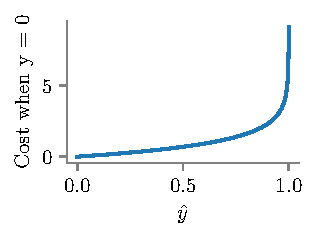
\includegraphics[scale=0.7]{../figures/logistic-regression/logistic-cross-cost-0}


\end{frame}

\begin{frame}
	Notebook: logits-usage
\end{frame}

\begin{frame}{Interpretation of Cross-Entropy Cost Function}\pause What is the interpretation of the cost function?



 $$J(\theta) = -y_i\log{\hat{y}_i} - (1-y_i)\log({1-\hat{y}_i})$$

\pause Now, assume $y_i$ is 1, then if $\hat{y}_i$ is 0, the loss is huge; but, if $\hat{y}_i$ is 1, the loss is zero!

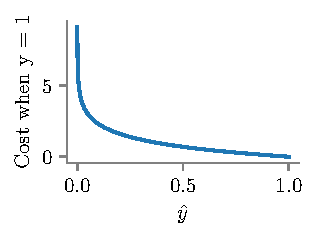
\includegraphics[scale=0.7]{../figures/logistic-regression/logistic-cross-cost-1}


\end{frame}

\begin{frame}{Cost function convexity}
\begin{columns}
	\begin{column}{0.5\textwidth}
		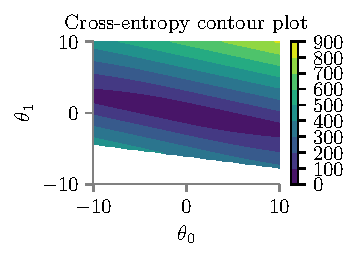
\includegraphics[scale=0.7]{../figures/logistic-regression/logistic-cross-loss-contour.pdf}
	\end{column}
	\begin{column}{0.5\textwidth}
		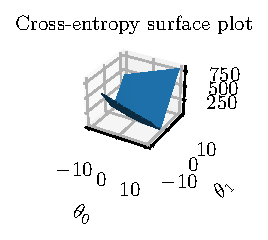
\includegraphics[scale=0.7]{../figures/logistic-regression/logistic-cross-loss-surface.pdf}
	\end{column}
\end{columns}
\end{frame}

\begin{frame}{Learning Parameters}
\begin{align*}
\frac{\partial J(\theta)}{\partial \theta_{j}} &= -\frac{\partial }{\partial \theta_{j}} \bigg\{\sum_{i=1}^{n} y_{i} log(\sigma_{\theta}(x_{i})) + (1 - y_{i})log(1 - \sigma_{\theta}(x_{i}))\bigg\} \\
&= -\sum_{i=1}^{n}\bigg[y_{i}\frac{\partial}{\partial \theta_{j}} \log(\sigma_{\theta}(x_{i})) + (1-y_{i})\frac{\partial}{\partial \theta_{j}} log(1 - \sigma_{\theta}(x_{i}))\bigg]
\end{align*}
\end{frame}
\begin{frame}{Learning Parameters}
\begin{align*}
\frac{\partial J(\theta)}{\partial \theta_{j}} &= -\sum_{i=1}^{n}\bigg[y_{i}\frac{\partial}{\partial \theta_{j}} \log(\sigma_{\theta}(x_{i})) + (1-y_{i})\frac{\partial}{\partial \theta_{j}} log(1 - \sigma_{\theta}(x_{i}))\bigg]
\end{align*}
\begin{align}
&= -\sum_{i=1}^{n}\bigg[\frac{y_{i}}{\sigma_{\theta}(x_{i})} \frac{\partial}{\partial \theta_{j}} \sigma_{\theta}(x_{i}) + \frac{1 - y_{i}}{1 - \sigma_{\theta}(x_{i})} \frac{\partial}{\partial \theta_{j}}(1 - \sigma_{\theta}(x_{i}))\bigg]
\end{align}
Aside:
\begin{equation*}
\frac{\partial}{\partial z}\sigma(z) = \frac{\partial}{\partial z}\frac{1}{1 + e^{-z}} = -(1 + e^{-z})^{-2}\frac{\partial}{\partial z}(1 + e^{-z})
\end{equation*}
\begin{equation*}
= \frac{e^{-z}}{(1 + e^{-z})^{2}} = \bigg(\frac{1}{1 + e^{-z}}\bigg)\bigg(\frac{e^{-z}}{1 + e^{-z}}\bigg) = \sigma(z)\bigg\{\frac{1 + e^{-z}}{1 + e^{-z}} - \frac{1}{1 + e^{-z}}\bigg\}
\end{equation*}
\begin{equation*}
\hspace{5.5cm}= \sigma(z)(1 - \sigma(z))
\end{equation*}
\end{frame}
\begin{frame}{Learning Parameters}
Resuming from (1)
\begin{equation*}
\frac{\partial J(\theta)}{\partial \theta_{j}} = -\sum_{i=1}^{n}\bigg[\frac{y_{i}}{\sigma_{\theta}(x_{i})} \frac{\partial}{\partial \theta_{j}} \sigma_{\theta}(x_{i}) + \frac{1 - y_{i}}{1 - \sigma_{\theta}(x_{i})} \frac{\partial}{\partial \theta_{j}}(1 - \sigma_{\theta}(x_{i}))\bigg]
\end{equation*}
\begin{equation*}
\hspace{-0.7cm}= -\sum_{i=1}^{n}\bigg[\frac{y_{i}\sigma_{\theta}(x_{i})}{\sigma_{\theta}(x_{i})}(1 - \sigma_{\theta}(x_{i}))\frac{\partial}{\partial \theta_{j}} (x_{i}\theta) + \frac{1 - y_{i}}{1 - \sigma_{\theta}(x_{i})}(1 - \sigma_{\theta}(x_{i})) \frac{\partial}{\partial \theta_{j}}(1 - \sigma_{\theta}(x_{i}))\bigg]
\end{equation*}
\begin{equation*}
= -\sum_{i=1}^{n}\bigg[y_{i}(1 - \sigma_{\theta}(x_{i}))x_{i}^{j} - (1 - y_{i})\sigma_{\theta}(x_{i})x_{i}^{j}\bigg]
\end{equation*}
\begin{equation*}
= -\sum_{i=1}^{n}\bigg[(y_{i} - y_{i}\sigma_{\theta}(x_{i}) - \sigma_{\theta}(x_{i}) + y_{i}\sigma_{\theta}(x_{i}))x_{i}^{j}\bigg]
\end{equation*}
\begin{equation*}
= \sum_{i=1}^{n}\bigg[\sigma_{\theta}(x_{i}) - y_{i}\bigg]x_{i}^{j}
\end{equation*}
\end{frame}
\begin{frame}{Learning Parameters}
\centering
\framebox{$\frac{\partial J(\theta)}{\theta_{j}} = \sum_{i=1}^{N}\big[\sigma_{\theta}(x_{i}) - y_{i}\big]x_{i}^{j}$} \\
\vspace{0.3cm}
Now, just use Gradient Descent!
\end{frame}

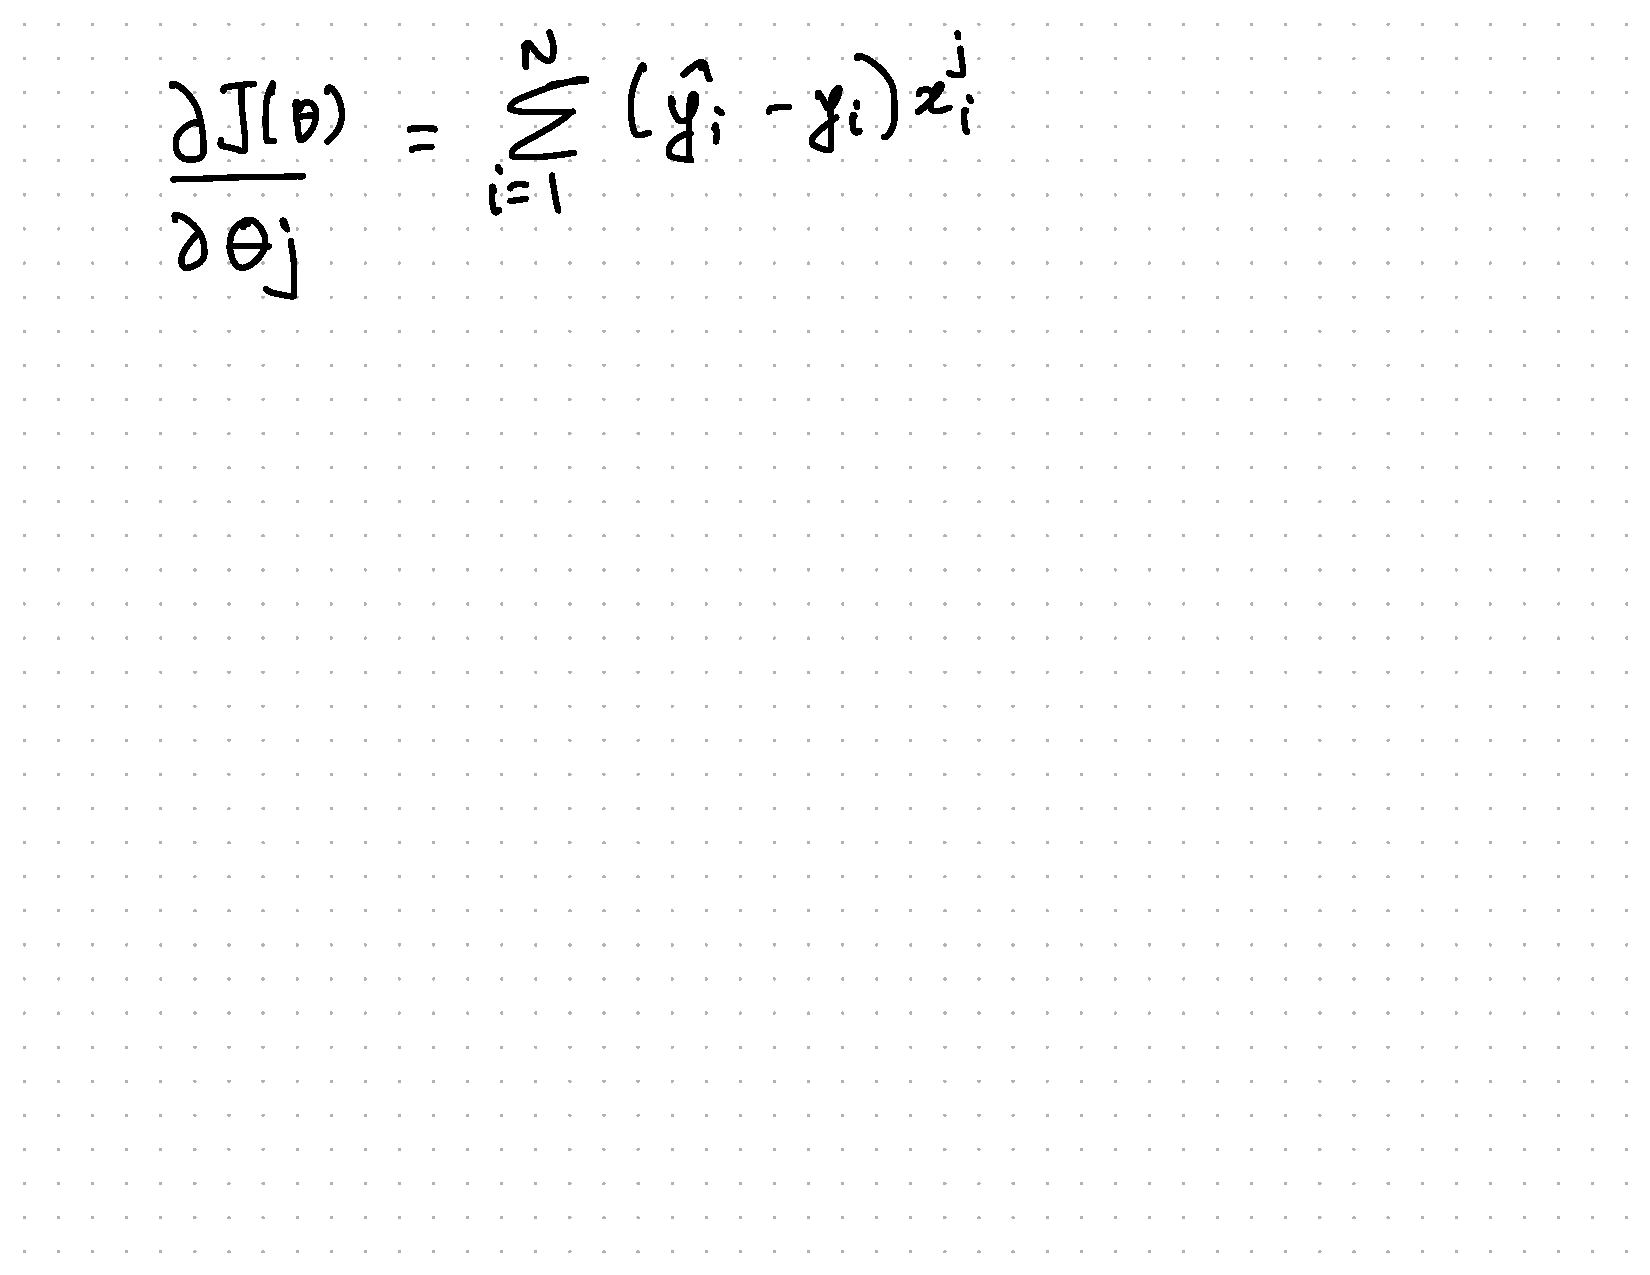
\includepdf[pages=-]{Logistic-vectorisation.pdf}

\begin{frame}{Logistic Regression with feature transformation}
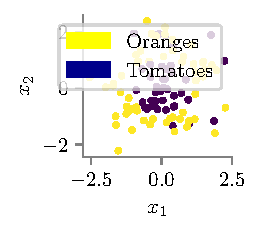
\includegraphics{../figures/logistic-regression/logisitic-circular-data.pdf}

What happens if you apply logistic regression on the above data?
\end{frame}


\begin{frame}{Logistic Regression with feature transformation}
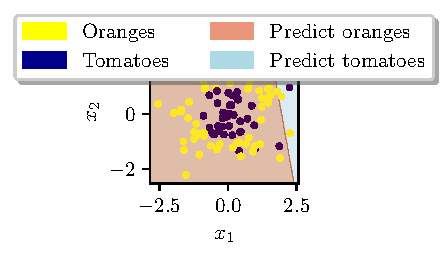
\includegraphics{../figures/logistic-regression/logisitic-linear-prediction.pdf}

Linear boundary will not be accurate here. What is the technical name of the problem?
\pause Bias! 
\end{frame}

\begin{frame}{Logistic Regression with feature transformation}
$$
\phi(x)=\left[\begin{array}{c}
{\phi_{0}(x)} \\
{\phi_{1}(x)} \\
{\vdots} \\
{\phi_{K-1}(x)}
\end{array}\right]=\left[\begin{array}{c}
{1} \\
{x} \\
{x^{2}} \\
{x^{3}} \\
{\vdots} \\
{x^{K-1}}
\end{array}\right] \in \mathbb{R}^{K}
$$
\end{frame}


\begin{frame}{Logistic Regression with feature transformation}
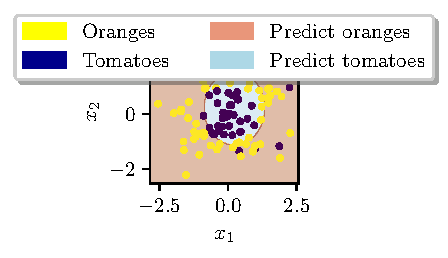
\includegraphics{../figures/logistic-regression/logisitic-circular-prediction.pdf}

Using $x_1^2, x_2^2$ as additional features, we are able to learn a more accurate classifier. 
\end{frame}

\begin{frame}{Logistic Regression with feature transformation}

How would you expect the probability contours look like?
\pause 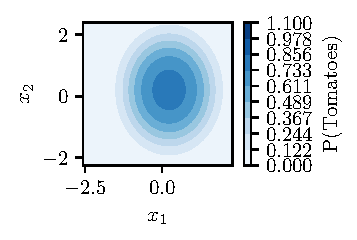
\includegraphics{../figures/logistic-regression/logisitic-circular-probability.pdf}


\end{frame}

\begin{frame}{Multi-Class Prediction}
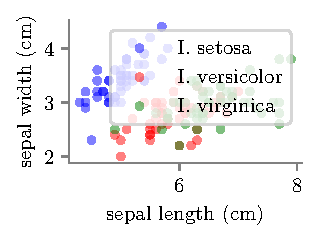
\includegraphics{../figures/logistic-regression/logisitic-iris.pdf}


\pause How would you learn a classifier? Or, how would you expect the classifier to learn decision boundaries?
\end{frame}

\begin{frame}{Multi-Class Prediction}
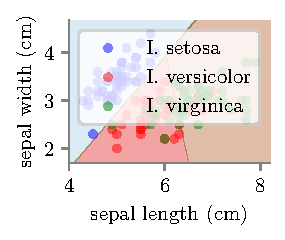
\includegraphics{../figures/logistic-regression/logisitic-iris-prediction.pdf}
\pause \begin{enumerate}
\item Use one-vs.-all on \underline{Binary} Logistic Regression
\item Use one-vs.-one on \underline{Binary} Logistic Regression
\item Extend \underline{Binary} Logistic Regression to \underline{Multi-Class} Logistic Regression
\end{enumerate}
\end{frame}

\begin{frame}{Multi-Class Prediction}
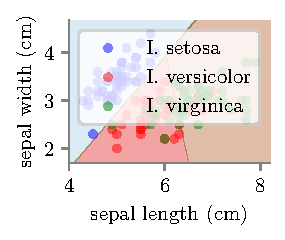
\includegraphics[scale=0.8]{../figures/logistic-regression/logisitic-iris-prediction.pdf}
\pause \begin{enumerate}
	\item Learn P(setosa (class 1)) = $\mathcal{F}({X\theta_1})$
	\item P(versicolor (class 2)) = $\mathcal{F}({X\theta_2})$
	\item P(virginica (class 3)) = $\mathcal{F}({X\theta_3})$
	\item Goal: Learn $\theta_i \forall i \in \{1, 2, 3\}$
	\item Question: What could be an $\mathcal{F}?$

\end{enumerate}


\end{frame}

\begin{frame}{Multi-Class Prediction}
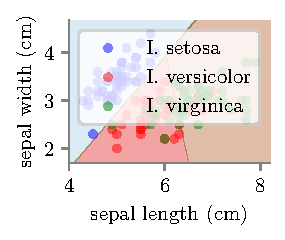
\includegraphics[scale=0.8]{../figures/logistic-regression/logisitic-iris-prediction.pdf}
\pause \begin{enumerate}
	\item Question: What could be an $\mathcal{F}?$
	\item Property: $\sum_{i=1}^{3}\mathcal{F}{({X\theta_i})} = 1$
	\item Also $\mathcal{F}(z)\in [0, 1]$
	\item Also, $\mathcal{F}(z)$ has squashing proprties: $R \mapsto [0, 1]$
\end{enumerate}


\end{frame}
\begin{frame}{Softmax}
\begin{equation*}
Z \in \mathbb{R}^{d}
\end{equation*}
\begin{equation*}
\mathcal{F}(z_{i}) = \frac{e^{z_{i}}}{\sum_{i=1}^{d}e^{z_{i}}}
\end{equation*}
\begin{equation*}
\therefore \sum \mathcal{F}(z_{i}) = 1
\end{equation*}

$\mathcal{F}(z_{i})$ refers to \underline{probability} of class \underline{i}
\end{frame}
\begin{frame}{Softmax for Multi-Class Logistic Regression}
\begin{equation*}
k = \{1, \ldots, k\} \text{classes}
\end{equation*}
$$
\theta=\left[\begin{array}{llll}
{\vdots} & {\vdots} & {\vdots} & {\vdots} \\
{\theta_{1}} & {\theta_{2}} & {\cdots} & {\theta_{k}} \\
{\vdots} & {\vdots} & {\vdots} & {\vdots} 	
\end{array}\right]
$$
\centering
\framebox{$P(y = k|X, \theta) = \frac{e^{X\theta_{k}}}{\sum_{k=1}^{K}e^{X\theta_{k}}}$}
\end{frame}
\begin{frame}{Softmax for Multi-Class Logistic Regression}
For K = 2 classes,
\begin{equation*}
P(y = k|X, \theta) = \frac{e^{X\theta_{k}}}{\sum_{k=1}^{K}e^{X\theta_{k}}}
\end{equation*}
\begin{equation*}
P(y = 0|X, \theta) = \frac{e^{X\theta_{0}}}{e^{X\theta_{0}} + e^{X\theta_{1}}}
\end{equation*}
\begin{equation*}
P(y = 1|X, \theta) = \frac{e^{X\theta_{1}}}{e^{X\theta_{0}} + e^{X\theta_{1}}} = \frac{e^{X\theta_{1}}}{e^{X\theta_{1}}\{1 + e^{X(\theta_{0} - \theta_{1})}\}}
\end{equation*}
\begin{equation*}
= \frac{1}{1 + e^{-X\theta^{'}}}
\end{equation*}
\begin{equation*}
= \text{Sigmoid!}
\end{equation*}
\end{frame}

\begin{frame}{Multi-Class Logistic Regression Cost}
Assume our prediction and ground truth  for the three classes for $i^{th}$ point is:
$$
\hat{y_i} = \begin{bmatrix}
	0.1\\0.8\\0.1
\end{bmatrix} = \begin{bmatrix}
\hat{y}_i^1\\\hat{y}_i^2\\\hat{y}_i^3
\end{bmatrix} 
$$

$$
y_i = \begin{bmatrix}
0\\1\\0
\end{bmatrix}=\begin{bmatrix}
y_i^1\\y_i^2\\ y_i^3
\end{bmatrix}
$$
meaning the true class is Class \#2

\pause Let us calculate $-\sum_{k=1}^{3}y_i^k \log{\hat{y}_i^k} $

\pause  = $-(0\times \log(0.1) + 1\times \log(0.8) + 0\times \log(0.1))$

\pause Tends to zero

\end{frame}

\begin{frame}{Multi-Class Logistic Regression Cost}
Assume our prediction and ground truth  for the three classes for $i^{th}$ point is:
$$
\hat{y_i} = \begin{bmatrix}
0.3\\0.4\\0.3
\end{bmatrix} = \begin{bmatrix}
\hat{y}_i^1\\\hat{y}_i^2\\\hat{y}_i^3
\end{bmatrix} 
$$

$$
y_i = \begin{bmatrix}
0\\1\\0
\end{bmatrix}=\begin{bmatrix}
y_i^1\\y_i^2\\ y_i^3
\end{bmatrix}
$$
meaning the true class is Class \#2

\pause Let us calculate $-\sum_{k=1}^{3}y_i^k \log{\hat{y}_i^k} $

\pause  = $-(0\times \log(0.1) + 1\times \log(0.4) + 0\times \log(0.1))$

\pause High number! Huge penalty for misclassification!

\end{frame}

\begin{frame}{Multi-Class Logistic Regression Cost}


For 2 class we had:
\begin{equation*}
J(\theta) = -\bigg\{\sum_{i=1}^{n}y_{i}\log(\sigma_{\theta}(x_{i})) + (1 - y_{i})\log(1 - \sigma_{\theta}(x_{i}))\bigg\}
\end{equation*}

\pause More generally, 
\pause \begin{equation*}
J(\theta) = -\bigg\{\sum_{i=1}^{n}y_{i}\log(\hat{y}_i) + (1 - y_{i})\log(1 - \hat{y}_i)\bigg\}
\end{equation*}

\pause \begin{equation*}
J(\theta) = -\bigg\{\sum_{i=1}^{n}y_{i}\log(\hat{y}_i) + (1 - y_{i})\log(1 - \hat{y}_i)\bigg\}
\end{equation*}

Extend to K-class:
\begin{equation*}
J(\theta) = -\bigg\{\sum_{i=1}^{n}\sum_{k=1}^{K}y_{i}^k\log(\hat{y}_{i}^k)\bigg\}
\end{equation*}
\end{frame}
\begin{frame}{Multi-Class Logistic Regression Cost}
\begin{equation*}
\text{Now:}
\end{equation*}
\begin{equation*}
\frac{\partial J(\theta)}{\partial \theta_{k}} = \sum_{i=1}^{n}\bigg[x_{i}\bigg\{I(y_{i} = k) - P(y_{i} = k | x_{i}, \theta)\bigg\}\bigg]
\end{equation*}
\end{frame}


\begin{frame}{Hessian Matrix}
The Hessian matrix of f(.) with respect to $\theta$, written $\nabla _{\theta}^{2}f(\theta)$ or simply as $\mathbb{H}$, is the $d \times d$ matrix of partial derivatives,
\begin{equation*}
\nabla _{\theta}^{2}f(\theta) = \begin{bmatrix} \frac{\partial^{2}f(\theta)}{\partial \theta_{1}^{2}} & \frac{\partial^{2}f(\theta)}{\partial \theta_{1}\partial \theta_{2}} & \ldots & \frac{\partial^{2}f(\theta)}{\partial \theta_{1}\partial \theta_{n}} \\ \frac{\partial^{2}f(\theta)}{\partial \theta_{2}\partial \theta_{1}} & \frac{\partial^{2}f(\theta)}{\partial \theta_{2}^{2}} & \ldots & \frac{\partial^{2}f(\theta)}{\partial \theta_{2}\partial \theta_{n}} \\ \ldots & \ldots & \ldots & \ldots \\ \ldots & \ldots & \ldots & \ldots \\ \frac{\partial^{2}f(\theta)}{\partial \theta_{n} \partial \theta_{1}} & \frac{\partial^{2}f(\theta)}{\partial \theta_{n}\partial \theta_{2}} & \ldots & \frac{\partial^{2}f(\theta)}{\partial \theta_{n}^{2}}\end{bmatrix}
\end{equation*}

\end{frame}
\begin{frame}{Newton's Algorithm}
The most basic second-order optimization algorithm is Newton's algorithm, which consists of updates of the form,

$$\theta_{k+1} = \theta_{k} - \mathbb{H}_{k}^{1}g_{k}$$
where $g_{k}$ is the gradient at step $k$. This algorithm is derived by making a second-order Taylor series approximation of $f(\theta)$ around $\theta_{k}$:
$$f_{quad}(\theta) = f(\theta_{k}) + g_{k}^{T}(\theta - \theta_{k}) + \frac{1}{2}(\theta - \theta_{k})^{T}\mathbb{H}_{k}(\theta - \theta_{k})$$
differentiating and equating to zero to solve for $\theta_{k+1}$.
\end{frame}
\begin{frame}{Learning Parameters}
Now assume:
$$g(\theta) = \sum_{i=1}^{n}\bigg[\sigma_{\theta}(x_{i}) - y_{i}\bigg]x_{i}^{j} = \mathbf{X^{T}(\sigma_{\theta}(X) - y)}$$
$$\pi_{i} = \sigma_{\theta}(x_{i})$$
Let $\mathbb{H}$ represent the Hessian of $J(\theta)$
\begin{align*}
\mathbb{H} = \frac{\partial}{\partial \theta} g(\theta) &= \frac{\partial}{\partial \theta} \sum_{i=1}^{n} \bigg[\sigma_{\theta}(x_{i}) - y_{i}\bigg]x_{i}^{j} \\
&= \sum_{i=1}^{n} \bigg[\frac{\partial}{\partial \theta}\sigma_{\theta}(x_{i})x_{i}^{j} - \frac{\partial}{\partial \theta} y_{i}x_{i}^{j}\bigg] \\
&= \sum_{i=1}^{n} \sigma_{\theta}(x_{i}) (1 - \sigma_{\theta}(x_{i}))x_{i}x_{i}^{T} \\
&= \mathbf{X^{T}}diag(\sigma_{\theta}(x_{i}) (1 - \sigma_{\theta}(x_{i})))\mathbf{X}
\end{align*}
\end{frame}
\begin{frame}{Iteratively reweighted least squares (IRLS)}
For binary logistic regression, recall that the gradient and Hessian of the negative log-likelihood are given by:
\begin{align*}
g(\theta)_{k} &= \mathbf{X^{T}(\pi_{k} - y)} \\
\mathbf{H}_{k} &= \mathbf{X}^{T}S_{k}\mathbf{X} \\
\mathbf{S}_{k} &= diag(\pi_{1k}(1 - \pi_{1k}), \ldots, \pi_{nk}(1 - \pi_{nk})) \\
\pi_{ik} &= sigm(\mathbf{x_{i}\theta_{k}})
\end{align*}
The Newton update at iteraion $k$ + 1 for this model is as follows:
\begin{align*}
\theta_{k+1} &= \theta_{k} - \mathbb{H}^{-1}g_{k} \\
&= \theta_{k} + (X^{T}S_{k}X)^{-1}X^{T}(y - \pi_{k}) \\
&= (X^{T}S_{k}X)^{-1}[(X^{T}S_{k}X)\theta_{k} + X^{T}(y - \pi_{k})] \\
&= (X^{T}S_{k}X)^{-1}X^{T}[S_{k}X\theta_{k} + y - \pi_{k}]
\end{align*}
\end{frame}
\begin{frame}{Regularized Logistic Regression}
Unregularised:
\begin{equation*}
J_{1}(\theta) = -\bigg\{\sum_{i=1}^{n}y_{i}\log(\sigma_{\theta}(x_{i})) + (1 - y_{i})\log(1 - \sigma_{\theta}(x_{i}))\bigg\}
\end{equation*}
L2 Regularization:
\begin{equation*}
J(\theta) = J_{1}(\theta) + \lambda\theta^{T}\theta
\end{equation*}
L1 Regularization:
\begin{equation*}
J(\theta) = J_{1}(\theta) + \lambda|\theta|
\end{equation*}
\end{frame}
\end{document}
